\Lecture{Jayalal Sarma}{Oct 21, 2020}{19}{Computing Ramsey Numbers and Multidimensional Ramsey numbers}{Shivlal Gangesh}{$\alpha$}{JS}
\section{Generalizing Ramsey numbers}
\begin{definition}[3-dimensional Ramsey numbers]
$R_3(p,q,r)$ is the minimum number $n$, such that any 3-edge coloring $K_n$ must have either a red $K_p$ or a blue $K_q$ or a green $K_r$
\end{definition}
\begin{definition}[$k$-dimensional Ramsey numbers]
$R_k(s_1,s_2,\cdots ,s_k)$ is the minimum number of vertices $n$ such that for any $k$-edge coloring of $K_n$  there must exist an $i$ such that there is a $K_{s_i}$ of colour $i$
\end{definition}

\section{Some Observations}
\begin{property}
$R(2,p)=p$
\end{property}
\begin{proof}
$ $ 
 \begin{description}
    \item[Case1 : $R(2,p) \leq p$]
    $ $ \newline
    Any 2-coloring of $K_p$ must have either a red $K_2$ or blue $K_p$. This is true because either there can exist a red edge (red $K_2$) or no red edge (blue $K_p$) in $K_p$
    \item[Case 2 : $R(2,p) \geq p$]
    $ $ \newline
    There exist a 2-coloring of edges of $K_{p-1}$ such that no red $K_2$ exists and no blue $K_p$ exists. Coloring all the edges of $K_{p-1}$ with blue will result in no red $K_2$ and no blue $K_p$ in $K_{p-1}$
 \end{description}
\end{proof}
\begin{claim}
$$ R(p,q) \leq {p+q-2 \choose p-1} $$
\end{claim}
\begin{proof}
 \begin{align*}
     R(p,q) &\leq  R(p,q-1) + R(p-1,q) && \textrm{(Erdos-Szekeres recurrence relation)} \\
     &\leq {p+(q-1)-2 \choose p-1} + {p-1+q-2 \choose p-2} \\
     &\leq {p+q-3 \choose p-1} + {p+q-3 \choose p-2} \\
     &\leq {p+q-2 \choose p-1}  && ({n+1 \choose k+1} = {n \choose k+1} +{n \choose k})
 \end{align*}

\end{proof}
\section{Explicit Computation of R(3,4)}
We don't know the exact values of Ramsey numbers for higher values as their computation becomes very hard. There is this famous saying by Paul Erdos on the difficulty of computing Ramsey numbers that
\begin{description}
   \item[Paul Erdos on Ramsey numbers] 
   $ $ \newline
\textit{   "Suppose aliens invade the earth and threaten to obliterate it in a year's time unless human beings can find the Ramsey number for red five and blue five. We could marshal the world's best minds and fastest computers, and within a year we could probably calculate the value. If the aliens demanded the Ramsey number for red six and blue six, however, we would have no choice but to launch a preemptive attack."}
\end{description}
 So let us now try to calculate the value of $R(3,4)$. 
 \begin{claim}
 $$ R(3,4) = 9 $$
 \end{claim}
 \begin{proof}
 $ $
 Consider any 2-coloring of $K_9$ and call it as $G$. We need to prove that $G$ has either a red $K_3$ or a blue $K_4$. Any vertex in $G$ can have it's incident edges as one of the three cases below
  \begin{itemize}
  \item \textbf{Case 1 : }There are at least $4$ red edges going out of the vertex
  \item \textbf{Case 2 : }There are at least $6$ blue edges going out of the vertex
  \item \textbf{Case 3 : }There are exactly $3$ red edges and $5$ blue edges going out of the vertex
  \end{itemize}
 However note that not all vertices in $G$ come under \textbf{Case 3} because, if so then the total sum of degrees of all vertices becomes odd which is not possible. So let $v$ be a vertex in $G$ which does not fall under \textbf{Case 3}. Then
 \begin{description}
    \item[Case 1 : There are at least 4 red edges going out of $v$ ]
    $ $ \newline
    Let $H_1$ be the subgraph of $G$ formed from the four vertices which are sharing the red edge with $v$.  Since we know that $R(2,4)=4$, $H_1$ with 4 vertices must have a red $K_2$ or a blue $K4$, So along with vertex $v$, $G$ must have a red $K_3$ or a blue $K_4$.
    \item[Case 2 :There are at least 6 blue edges going out of $v$]
    $ $ \newline
    Let $H_2$ be the subgraph of $G$ formed from the six vertices which are sharing the blue edge with $v$. Since we know that $R(3,3)=6$, $H_2$ with 6 vertices must have a red $K_3$ or a blue $K3$, So along with vertex $v$, $G$ must have a red $K_3$ or a blue $K_4$.
    \item[Proof for tightness]
    $ $ \newline
    To prove that $9$ is tight, we need to show that there is a 2-coloring of $K_8$ such that it does not have red $K_3$ or blue $K_4$. Given below is one such  example
\begin{figure}[h!]
    \centering
    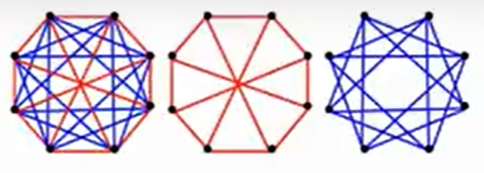
\includegraphics[width=0.5\linewidth]{images/R34counter_example.png}
    \caption{2-coloring of $K_8$ with no red $K_3$ and no blue $K_4$}
\end{figure}
 \end{description}
  
 \end{proof}
 As the values $p$, $q$ increases we can only calculate the range of the Ramsey number. The following is a table with value or range of Ramsey numbers for the first few natural numbers.
 \begin{figure}[h!]
    \centering
    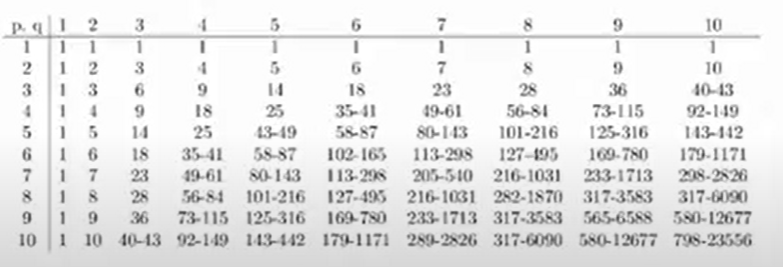
\includegraphics[width=1\linewidth]{images/RamseyTable.png}
    \caption{Table for $R(p,q)$}
\end{figure}